\documentclass[10pt]{article}


%---------- Uncomment one of them ------------------------------
\usepackage[includeheadfoot, top=1in, bottom=1in, hmargin=1in]{geometry}

% \usepackage[a5paper, landscape, twocolumn, twoside,
%    left=2cm, hmarginratio=2:1, includemp, marginparwidth=43pt,
%    bottom=1cm, foot=.7cm, includefoot, textheight=11cm, heightrounded,
%    columnsep=1cm, dvips,  verbose]{geometry}
%---------------------------------------------------------------
\usepackage{fancyhdr}
\usepackage{verbatim}
\usepackage{url}
\usepackage{epsfig}
\pagestyle{fancy}
\usepackage{setspace}
\usepackage{amsmath}
\usepackage{graphicx}


\pdfpagewidth 8.5in
\pdfpageheight 10in 
%\doublespacing
\singlespacing
%\onehalfspacing

\lhead{Astronomy Lab 6}
\chead{}
\rhead{Week 6}
\lfoot{Joseph}
\cfoot{\thepage}
\rfoot{Fall 2026}


\begin{document}

\begin{center}
{\Huge Lab 7: The Moon}   %;;;;;;;;;;;;;;;
\end{center}

\begin{flushleft}
\vspace{0.3in}
\section*{Part I--- Rules of Thumb}
\subsection*{Calibrate your hand to measure angles}
\vspace{0.1in}
\paragraph{}
The apparent positions and separations of objects in the sky are not determined by the linear distances between two objects but by their angular separation. For example, the angular distance from the horizon to directly overhead, the zenith, is $90^\circ$. Not only can we measure the angular separation between two objects, but we can also measure the angular size of an object such as the Moon, the Sun, and galaxies. Sextants allow the precise measurement of angles, but not all of us carry one in our back pocket (plus they take some practice). Luckily, there is a \textsl{handy} way to measure angular size. 

\paragraph{}
Hold your arm out straight in front of you. Now extend your thumb like you're hitchhiking. This will be one of your basic measuring devices. Now make a loose fist. There's your other device.

\vspace{0.2in}
\subsection*{Record all your measurements and your calculations in your notebook}

\paragraph{}
Measure the width of your thumb across the nail. Use the string to
measure the distance from your eye to your thumb at arm's length. Get
as accurate a measurement as possible. Calculate the angle subtended by your thumb in
degrees.

\paragraph{}
Repeat this process for your fist (across the knuckles)

\paragraph{}
You now have two ``devices'' for estimating angles that are always
with you.  Use both of them to measure the angular size of a 2 things in the room.  Pick 1 not-too-big object and measure its angular size with both your fist and your thumb.  Then measure the distance from you to the object, and its actual size.  Use these to calculate the angular size as well, and check how close your measurements are to reality.  Why might your measurement be inaccurate? 

\vspace{0.3in}
\section*{Part II--- The Moon}

\begin{figure*}
    \centering
    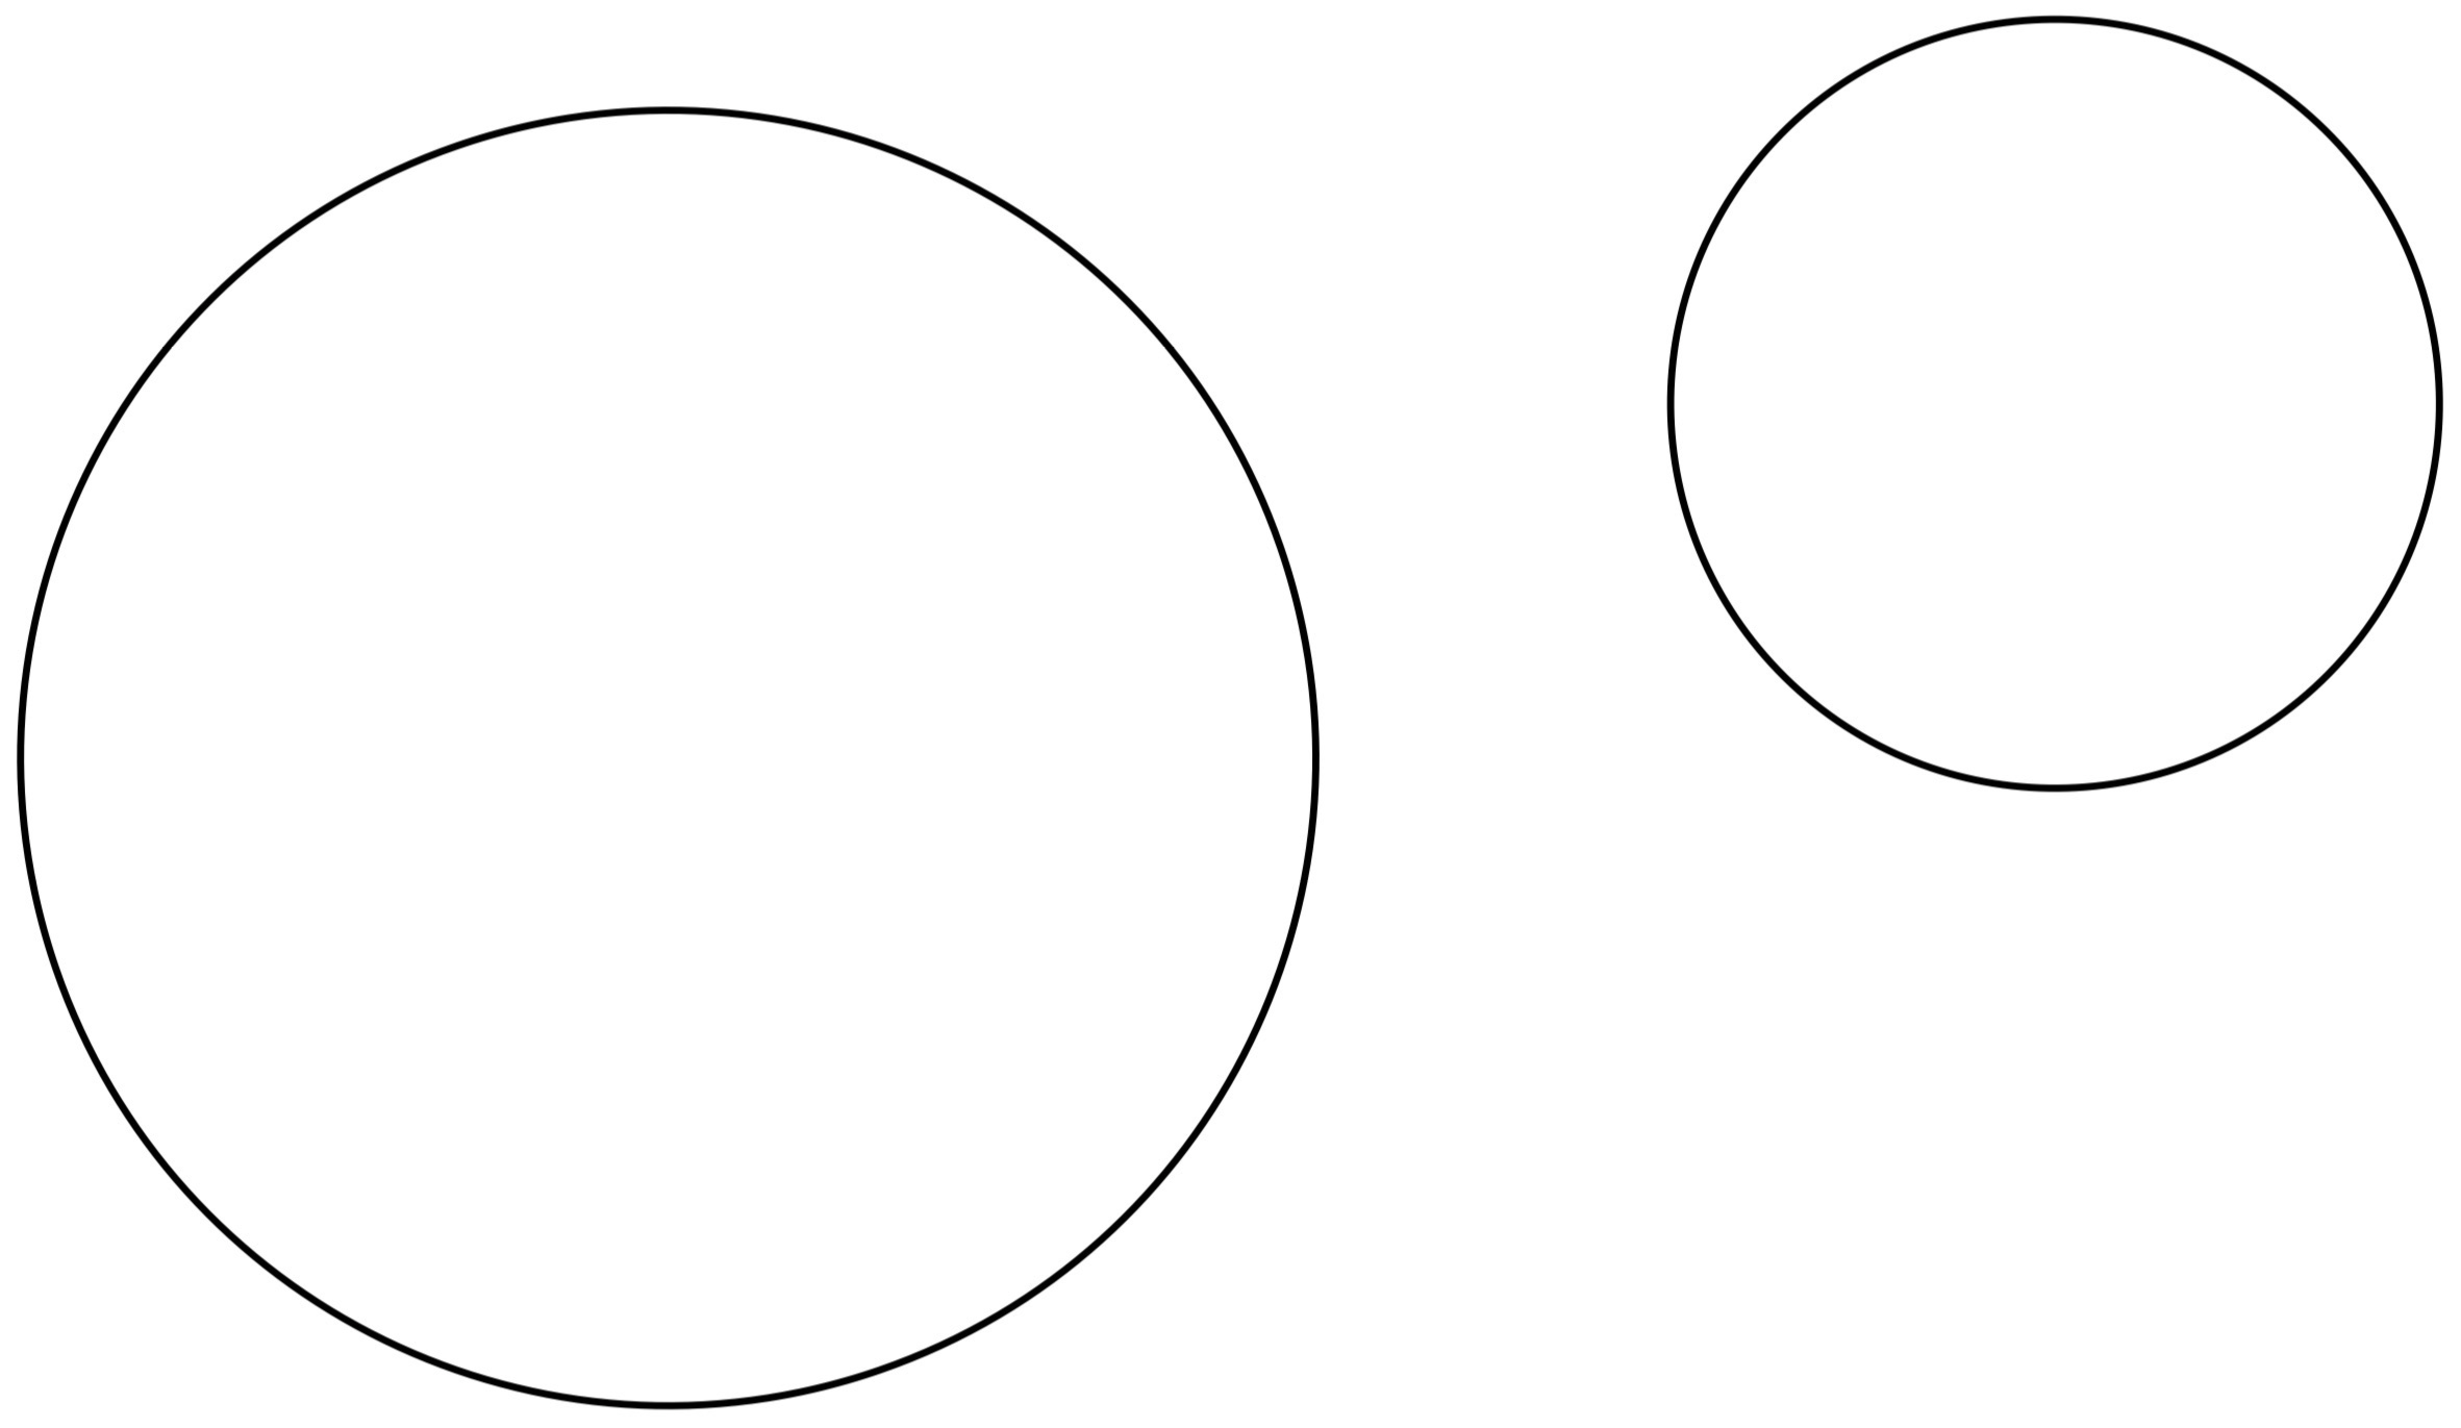
\includegraphics[width=0.75\linewidth]{moon_sketch.pdf}
    \caption{Your sketch of the Moon. The circle on the left is for the large field of view, and the circle on the right is the smaller field of view. Draw lines to indicate what region of the Moon you are zooming in on.}
    \label{fig:Moon sketch}
\end{figure*}
\subsection*{Draw a Portrait of the Moon}
\vspace{0.1in}
\paragraph{}

When we get up on the roof, Make two sketches of the Moon in Figure~\ref{fig:Moon sketch}:

\begin{itemize}
\item{One with a large field of view, so the whole disk is visible}
\vspace{0.1in}
\item{One with a small field of view, focusing on one section.  Indicate on the larger drawing where you zoomed in for the close up drawing.}
\end{itemize}

\vspace{.05in}
\textbf{Also answer the following questions while you are on the roof or after:}

\begin{enumerate}
    \item Note the time.  How many degrees above the horizon is the Moon?  Use your fists to measure.

    \item How many degrees across is the Moon?  Use your thumb to measure.

    \item What is the radius of the Moon if it is 384,400 km away?

% \vspace{.05in}
% 3.  What do you notice about the craters?  Are there more or fewer than on Earth?  Does the surface directly adjacent to a crater look different?  How so and why do you think this might be?  How about the dark areas?  What do they look like up close?

    \item What do you notice about the shadows?  Can you find any craters with very large shadows compared to the size of the crater?  What does this say about the height of the crater edge?

    \item What kind of Moon is it?  (i.e. Full, New, Waxing Gibbous?  There is only one correct answer) Where is the sun?  Draw a picture if necessary.
\end{enumerate}


\vspace{0.2in}
\subsection*{Your own picture of the Moon!}
\vspace{0.2in}
\paragraph{}
The telescope in the little dome is set up with a digital SLR camera to take pictures of the Moon.  The telescope tracks with the sky so your pictures won't appear blurry.  Select one region of the Moon (maybe the part which you focused on in your drawing, or at the terminator, or the edge are all interesting) and take a picture of it.
\vspace{.1in}

We will note down which picture is yours and e-mail you your own Moon picture later this week!
\vspace{.2in}

%Before we head downstairs, re-measure the altitude of the Moon above the horizon and note the time. 

%\vspace{0.2in}

%\vspace{0.1in}

%Based on the change in the Moon's altitude while we were outside, and using the same formula ($\Delta RA = \Delta Alt / \cos(lat)$), calculate the time tonight when the Moon will set.

%\vspace{0.1in}

%Take a look at the Moon map at the front.  Try to identify four or five key features from your drawing of the large field of view and label them.  Also try to find a label for the most prominent feature from your small drawing.

% \vspace{0.2in}


% Any theory which explains the existence of the Moon must naturally explain the following facts:
% \begin{enumerate}
% \item The Moon's low density (3.3 $g/cm^3$) shows that it does not have a substantial iron core like the Earth does.
% \item Moon rocks contain few volatile substances (e.g. water), which implies extra baking of the lunar surface relative to that of Earth.
% \item The relative abundance of oxygen isotopes on Earth and on the Moon are identical, which suggests that the Earth and Moon formed at the same distance from the Sun.
% \end{enumerate}


\vspace{0.3in}

\section*{Part III --- Phases of the Moon}
For this activity, you will work in pairs and in the dark. You will try to model the Sun-Earth-Moon system. Every group will be assigned a Sun (flashlight) and a Moon (a ping-pong ball). One student is sitting on a chair corresponding to the observer on the Earth (student-Earth). The other student will use a flashlight to shed light on the Earth-Moon system (student-Sun). The student holding the Moon (student-Moon) will rotate around the student-Earth counterclockwise until they complete a full circle. The student-Earth must follow the rotation of the student-Moon by turning their chair around and observing what they see on the Moon. Which part of your Moon is bright and which is
dark?

\begin{enumerate}
    \item  In Figure~\ref{fig:Phases of the Moon}, sketch the shape of the Moon (as seen from the Earth). Make to clearly mark which part of the Moon is dark and which part of the Moon is bright.
    \item Can you recognize the phases of the Moon? Which configuration gives a Full Moon? Which gives a New Moon (when you cannot see the Moon)? Indicate them in your diagram.
    \item It takes the Moon 28 days to go around once. Let day 1 be the day of the New Moon. Note in the diagram which days correspond to each phase.
    \item It takes about 28 days for the Moon to orbit the Earth, but closer to 30 days for a new Moon to occur. Why does this happen?
    \item  What is the phase of the Moon during a solar eclipse? During a lunar eclipse? Why don’t they happen every month? Hint: You need perfect alignment. 

\end{enumerate}

\begin{figure*}
    \centering
    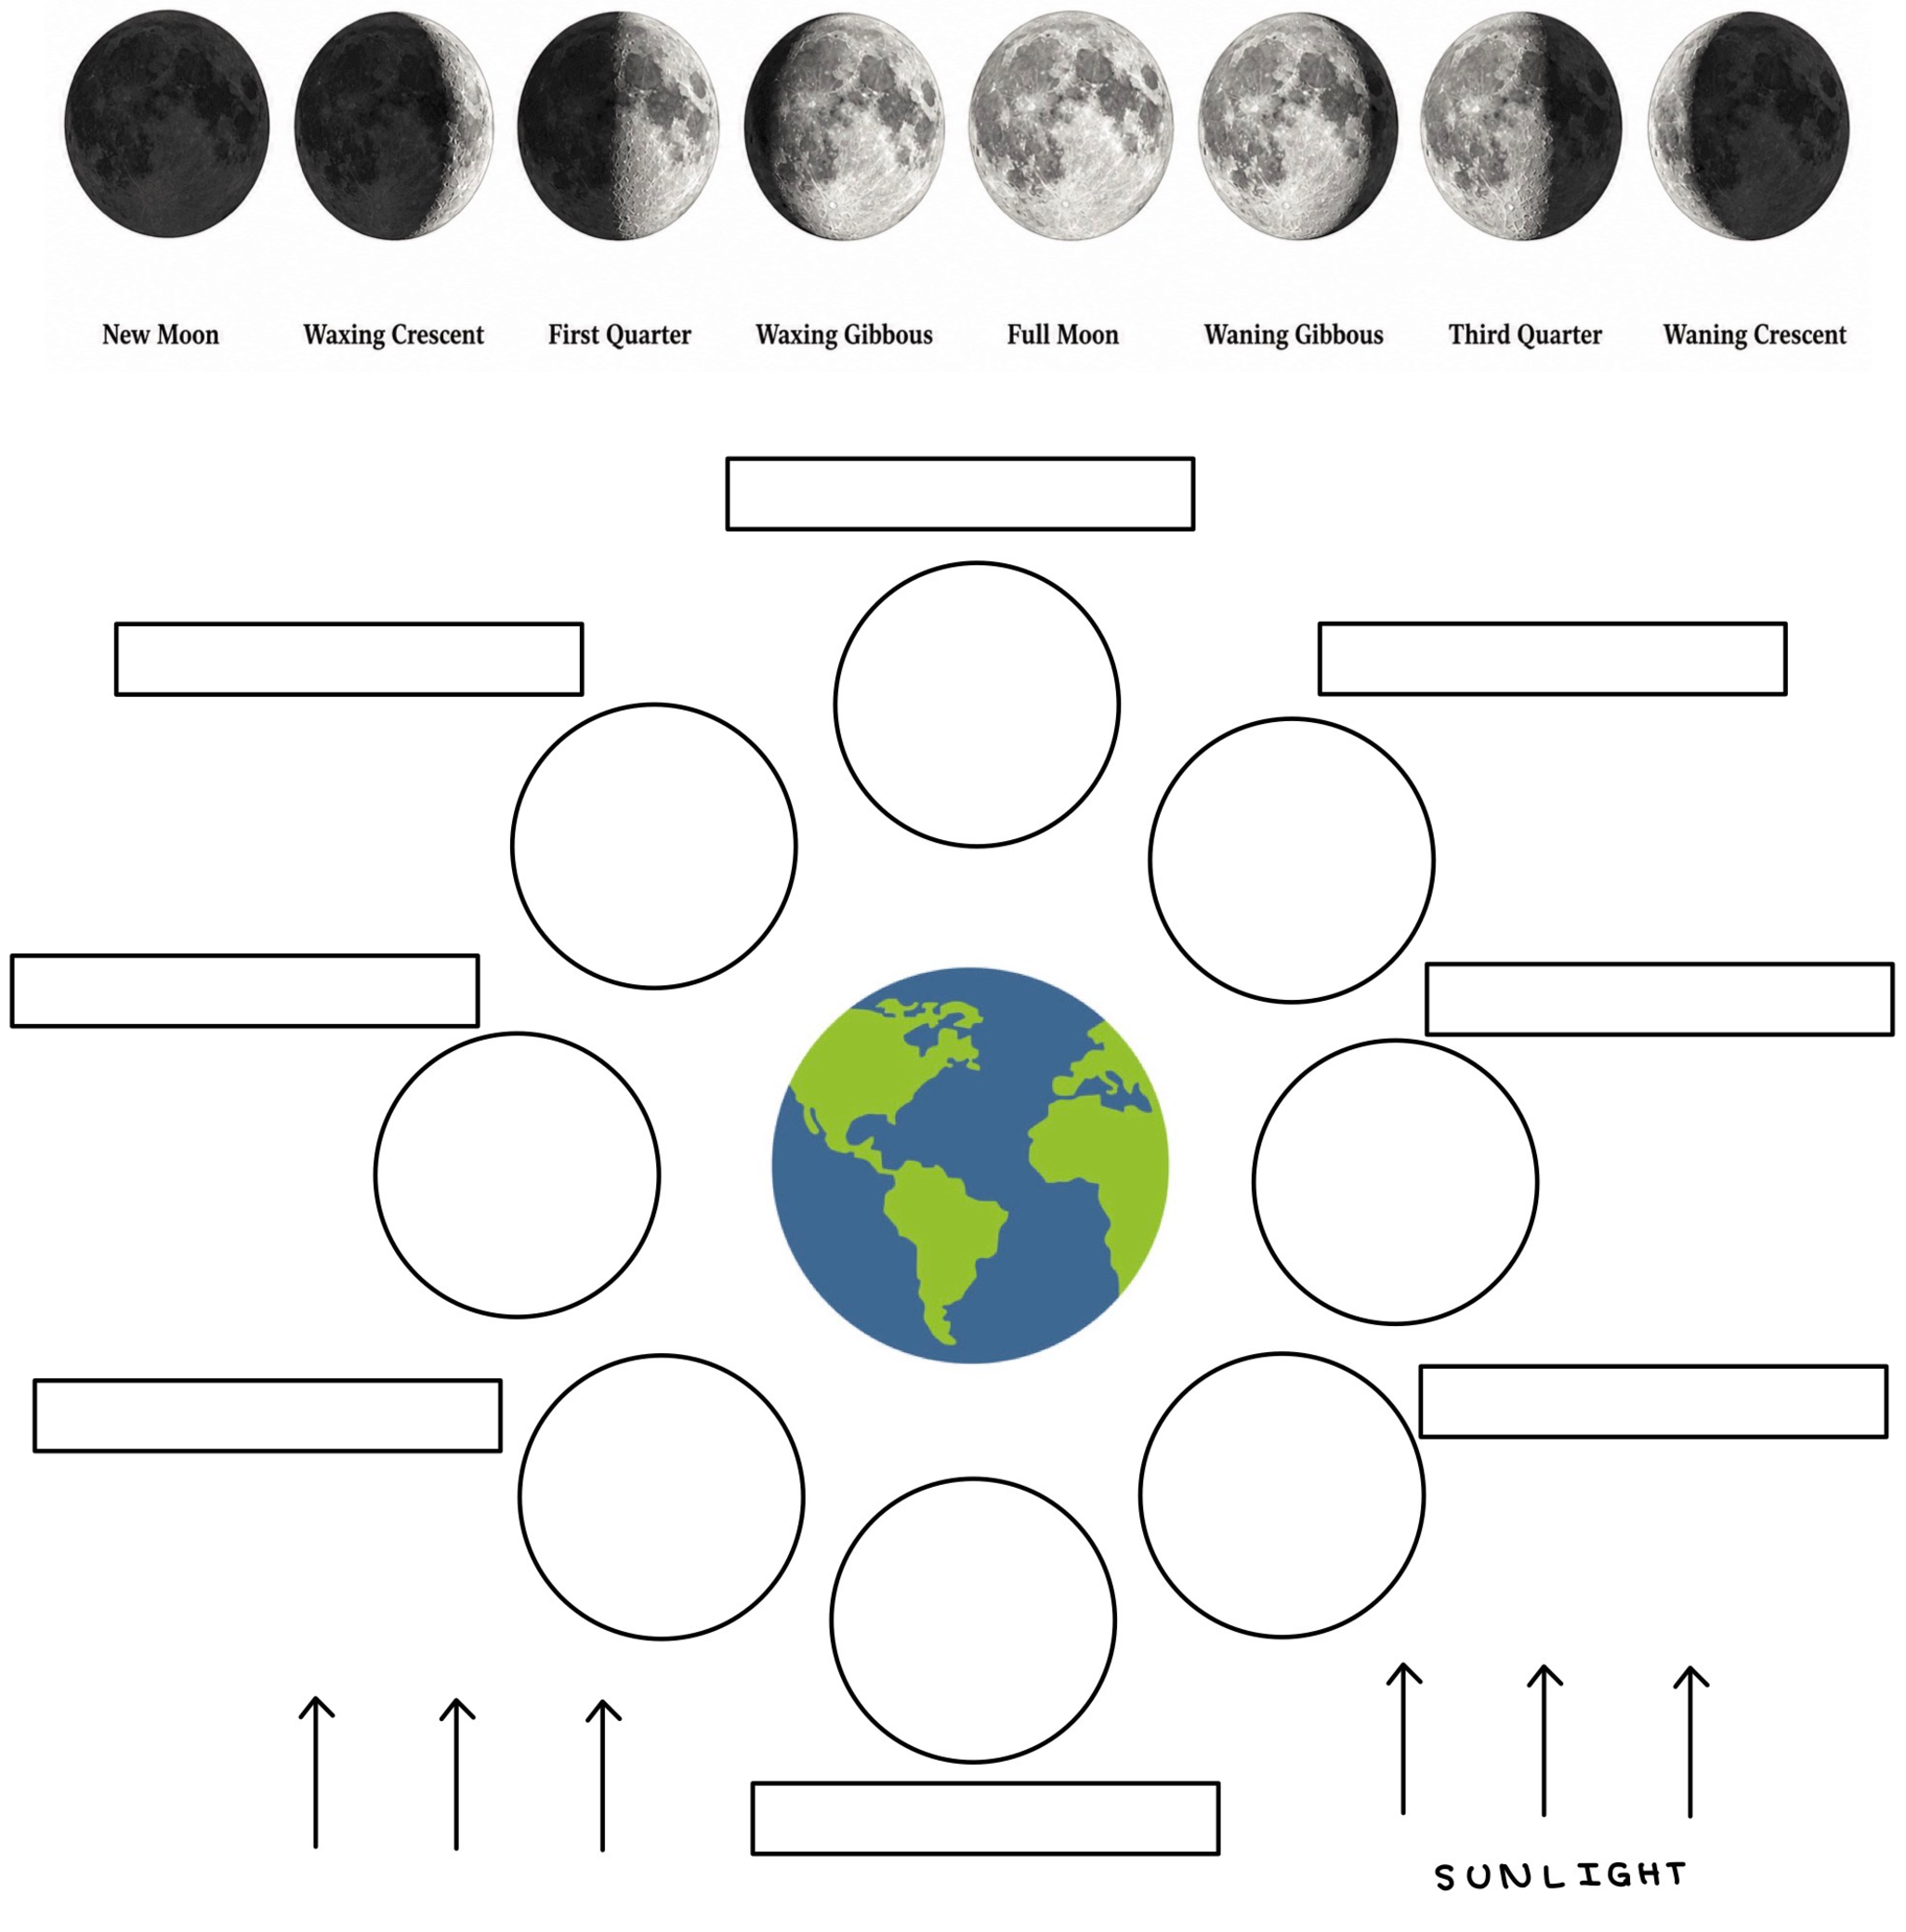
\includegraphics[width=0.95\linewidth]{moon_diagram.pdf}
    \caption{Phases of the Moon diagram. Sketch and label each phase of the Moon observed from Part III of the lab.}
    \label{fig:Phases of the Moon}
\end{figure*}

\section*{Part IV --- The Far Side of the Moon}

The far side of the Moon, sometimes called the “dark side of the Moon”, is the lunar hemisphere that permanently faces away from the Earth. It is therefore not visible from the Earth’s surface. The far hemisphere was first photographed by the Soviet Luna 3 probe in 1959, and was first directly observed by human eyes when the Apollo 8 mission orbited the Moon in 1968. Some conspiracy theorists have alleged that some Apollo astronauts had seen UFOs on the far side of the Moon but were told to keep quiet about them. Let’s see why we can’t see this mysterious side of the Moon. We always see the same side of the Moon. Why? Now repeat the previous experiment, but one student is the Moon, the other the Earth and the last one is a far observer standing outside the circle the Moon makes around the Earth. As the Moon rotates around the Earth, the student-Moon should always face the Earth. 

\begin{enumerate}
    \item Stand outside of the circle your classmate-Moon makes around Earth. Observe your classmate. Does the Moon rotate? Do you see the same side all the time? If not, what portion of the circle does she have to walk before you see the same side?
    \item Why do we always see the same side of the Moon? Think about how long it takes for the Moon to complete one orbit around the Earth and how long it takes for the Moon to rotate once about its axis.
    \item Why does the far side of the Moon have more craters?
\end{enumerate}


\section{Part V --- Tides}

Both the Sun and the Moon exert gravitational force to the Earth. The Sun is more massive, but the Moon is much closer. Go to (Note: You have a 5 minute timer on the page; try using an incognito tab :D) \\

\hspace{0.5in}\url{https://gizmos.explorelearning.com/find-gizmos/lesson-info?resourceId=368} \\

Use the animation to understand how the gravitational pull of the Moon changes the level of the sea during the day. Explain which configuration of the Sun-Earth-Moon system gives the most extreme tides (highest high tide and lowest low tide). Sketch a diagram of the Sun-Earth-Moon system during the spring and neap tides.



% \vspace{0.1in}


% \vspace{0.3in}
% \section*{Part III--- Outdoor Observing}
% \vspace{0.1in}

% Next we will estimate the number of stars that we can't see by being in New York City. Look directly overhead and find Vega.  Next to Vega will be the constellation Cygnus (the swan). Spend a minute or two letting your eyes adjust while looking up.  Decide which of the star charts at the right edge of the paper most closely corresponds to the view that you see.  Write this number down, and draw a brief sketch of how the sky around Cygnus looks.

% \vspace{0.2in}

% In this field of view, one can potentially see 14,000 stars.  About how many do you think you can count?  In general, the fainter the stars that you can see, the more you can see.  They follow the following trend:

% \begin{center}
% \begin{tabular}{|c|c|}
% \hline
% Limiting & Number\\
% Magnitude & Of Stars\\
% \hline
% 1 & 6\\
% 2 & 45\\
% 3 & 150\\
% 4 & 540\\
% 5 & 1700 \\
% 6 & 4900\\
% 7 & 14000\\
% \hline
% \end{tabular}
% \end{center}

% Based on the magnitude chart you picked above, how many stars were you NOT able to see tonight because of the lights of the city?  Where did you grow up?  Can you guess about what limiting magnitude the sky by your hometown is?  How many more stars can you see there than in New York City?


\end{flushleft} 

\end{document}
